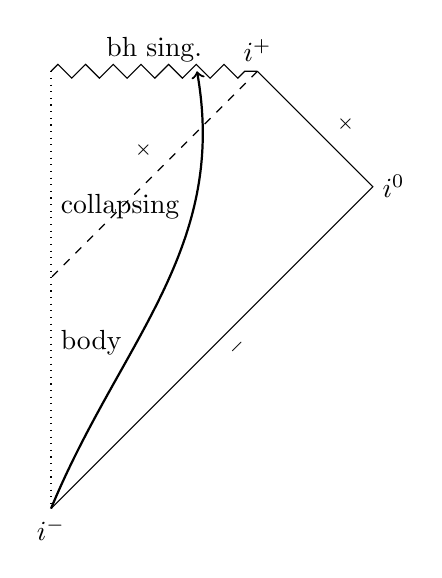
\begin{tikzpicture}%[scale=2]
\pgfmathsetmacro\myunit{3} 
\pgfmathsetmacro\sc{1.41421 35623 73095 04880 16887 24209 69807 85696 71875}
\pgfmathsetmacro\grs{0.6180339887498949}
\pgfmathsetmacro\grb{1.6180339887498949}
	\draw [decorate, decoration=zigzag] (0,0)
		-- ++ (+  0: \sc * \grs * \myunit)
			node [above] {$i^+$}
			node [pos = .5, above] {bh sing.}
			coordinate (i+);
	\draw [dotted] (0,0)
			\pgfextra{\pgfmathparse{(\grs/\sc+\sc)*\myunit}}
		-- ++ (- 90: \pgfmathresult)
			node [below] {$i^-$}
			node [pos = .31, right] {collapsing}
			node [pos = .62, right] {body}
			coordinate (i-);
	\draw (i+)
		\pgfextra{\pgfmathparse{(1 - \grs/2)*\myunit}}
		-- ++ (- 45: \pgfmathresult)
			node [right] {$i^0$}
			node [pos = .5, above right, sloped] {$\mscrI^+$}
			coordinate (i0)
		-- (i-)
			node [pos = .5, below right, sloped] {$\mscrI^-$};
	\draw [dashed] (i+)
		-- ++ (-135: 2 * \grs * \myunit)
			node [pos = .4, above left, sloped] {$\mscrh^+$};
	\draw [thick, out = 67.5, in = -80, thick, ->] (i-)
			to (\grs * \myunit, 0);
\end{tikzpicture}
